\documentclass{standalone}
\usepackage{tikz}
\usetikzlibrary{patterns, positioning}

\begin{document}
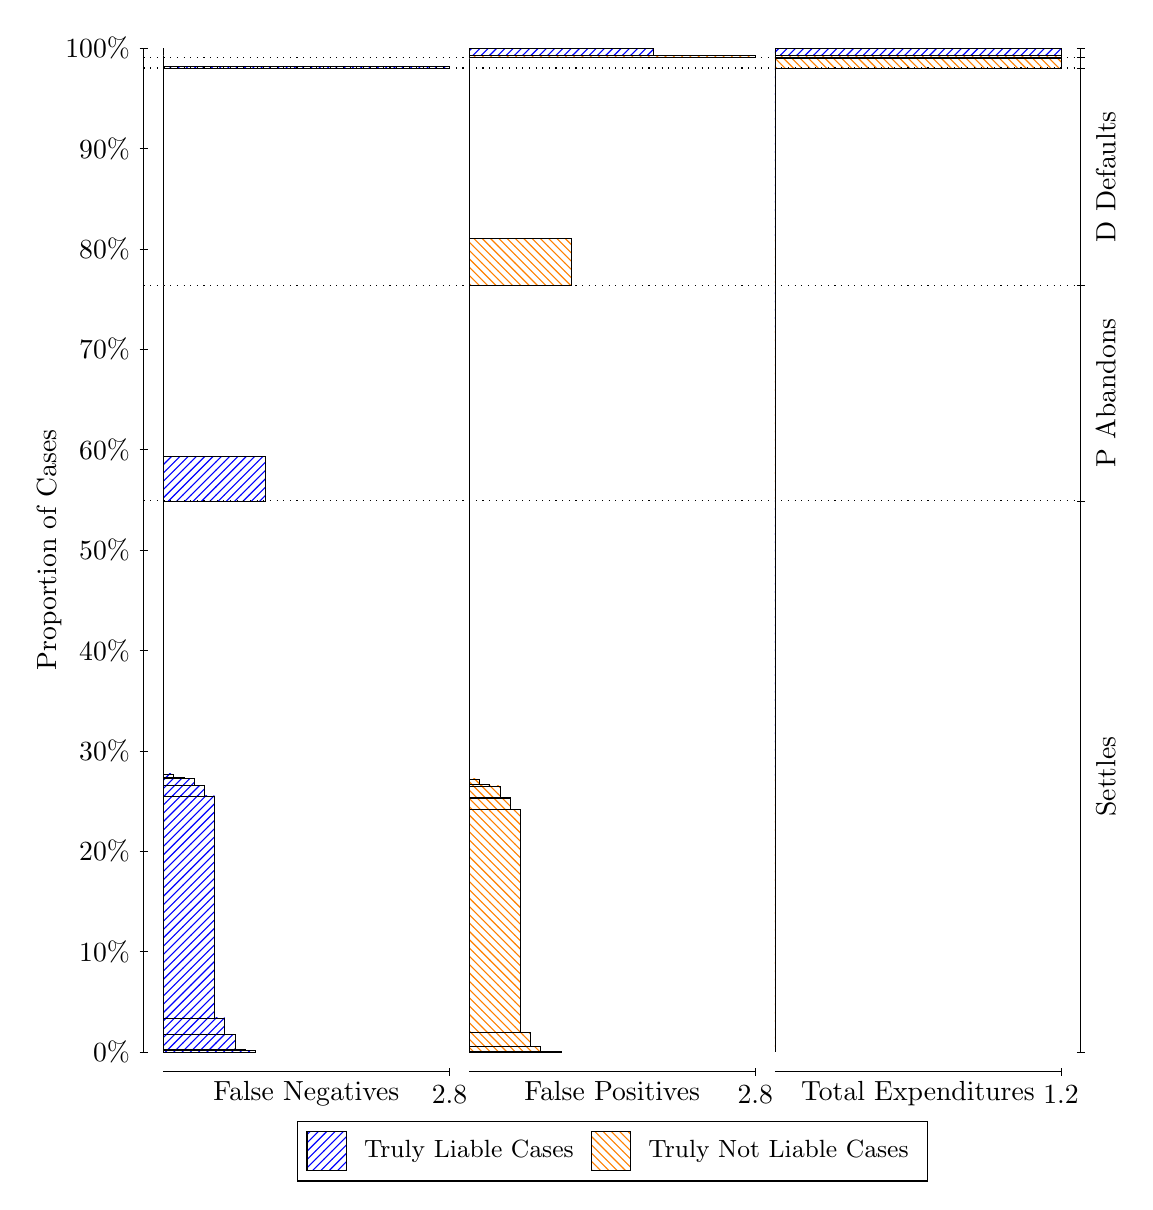
\begin{tikzpicture}
\draw[black, very thin] (1.5,1.75) -- (1.5,14.5);
\node[rotate=90, anchor=center] at (0.3, 8.125) {Proportion of Cases};
\draw[black, very thin] (1.45,1.75) -- (1.55,1.75);
\node[anchor=east] at (1.45, 1.75) {0\%};
\draw[black, very thin] (1.45,3.025) -- (1.55,3.025);
\node[anchor=east] at (1.45, 3.025) {10\%};
\draw[black, very thin] (1.45,4.3) -- (1.55,4.3);
\node[anchor=east] at (1.45, 4.3) {20\%};
\draw[black, very thin] (1.45,5.575) -- (1.55,5.575);
\node[anchor=east] at (1.45, 5.575) {30\%};
\draw[black, very thin] (1.45,6.85) -- (1.55,6.85);
\node[anchor=east] at (1.45, 6.85) {40\%};
\draw[black, very thin] (1.45,8.125) -- (1.55,8.125);
\node[anchor=east] at (1.45, 8.125) {50\%};
\draw[black, very thin] (1.45,9.4) -- (1.55,9.4);
\node[anchor=east] at (1.45, 9.4) {60\%};
\draw[black, very thin] (1.45,10.675) -- (1.55,10.675);
\node[anchor=east] at (1.45, 10.675) {70\%};
\draw[black, very thin] (1.45,11.95) -- (1.55,11.95);
\node[anchor=east] at (1.45, 11.95) {80\%};
\draw[black, very thin] (1.45,13.225) -- (1.55,13.225);
\node[anchor=east] at (1.45, 13.225) {90\%};
\draw[black, very thin] (1.45,14.5) -- (1.55,14.5);
\node[anchor=east] at (1.45, 14.5) {100\%};

\draw[black, very thin] (13.4,1.75) -- (13.4,14.5);
\draw[black, very thin] (13.35,1.75) -- (13.45,1.75);
\node[anchor=west] at (13.35, 1.75) {};
\draw[black, very thin] (13.35,8.75) -- (13.45,8.75);
\node[anchor=west] at (13.35, 8.75) {};
\draw[black, very thin] (13.35,11.486) -- (13.45,11.486);
\node[anchor=west] at (13.35, 11.486) {};
\draw[black, very thin] (13.35,14.247) -- (13.45,14.247);
\node[anchor=west] at (13.35, 14.247) {};
\draw[black, very thin] (13.35,14.385) -- (13.45,14.385);
\node[anchor=west] at (13.35, 14.385) {};
\draw[black, very thin] (13.35,14.5) -- (13.45,14.5);
\node[anchor=west] at (13.35, 14.5) {};

\draw[black, very thin, pattern color=blue, pattern=north east lines] (1.75,1.75) rectangle (2.9179,1.7676);
\draw[black, very thin, pattern color=blue, pattern=north east lines] (1.75,1.7676) rectangle (2.7881,1.7803);
\draw[black, very thin, pattern color=blue, pattern=north east lines] (1.75,1.7803) rectangle (2.6583,1.9707);
\draw[black, very thin, pattern color=blue, pattern=north east lines] (1.75,1.9707) rectangle (2.5286,1.9778);
\draw[black, very thin, pattern color=blue, pattern=north east lines] (1.75,1.9778) rectangle (2.5286,2.1824);
\draw[black, very thin, pattern color=blue, pattern=north east lines] (1.75,2.1824) rectangle (2.3988,5.0037);
\draw[black, very thin, pattern color=blue, pattern=north east lines] (1.75,5.0037) rectangle (2.269,5.1335);
\draw[black, very thin, pattern color=blue, pattern=north east lines] (1.75,5.1335) rectangle (2.1393,5.2244);
\draw[black, very thin, pattern color=blue, pattern=north east lines] (1.75,5.2244) rectangle (2.0095,5.2394);
\draw[black, very thin, pattern color=blue, pattern=north east lines] (1.75,5.2394) rectangle (1.8798,5.2804);
\draw[black, very thin, pattern color=orange, pattern=north west lines] (1.75,5.2804) rectangle (1.75,8.75);
\draw[black, very thin, pattern color=blue, pattern=north east lines] (1.75,8.75) rectangle (3.0476,9.3176);
\draw[black, very thin, pattern color=orange, pattern=north west lines] (1.75,9.3176) rectangle (1.75,11.486);
\draw[black, very thin, pattern color=orange, pattern=north west lines] (1.75,11.486) rectangle (1.75,12.085);
\draw[black, very thin, pattern color=blue, pattern=north east lines] (1.75,12.085) rectangle (1.75,14.247);
\draw[black, very thin, pattern color=blue, pattern=north east lines] (1.75,14.247) rectangle (5.3833,14.267);
\draw[black, very thin, pattern color=orange, pattern=north west lines] (1.75,14.267) rectangle (1.75,14.385);
\draw[black, very thin, pattern color=orange, pattern=north west lines] (1.75,14.385) rectangle (1.75,14.405);
\draw[black, very thin, pattern color=blue, pattern=north east lines] (1.75,14.405) rectangle (1.75,14.5);
\draw[black, very thin, pattern color=orange, pattern=north west lines] (5.6333,1.75) rectangle (6.8012,1.7554);
\draw[black, very thin, pattern color=orange, pattern=north west lines] (5.6333,1.7554) rectangle (6.6714,1.76);
\draw[black, very thin, pattern color=orange, pattern=north west lines] (5.6333,1.76) rectangle (6.5417,1.823);
\draw[black, very thin, pattern color=orange, pattern=north west lines] (5.6333,1.823) rectangle (6.4119,2.0012);
\draw[black, very thin, pattern color=orange, pattern=north west lines] (5.6333,2.0012) rectangle (6.2821,4.8307);
\draw[black, very thin, pattern color=orange, pattern=north west lines] (5.6333,4.8307) rectangle (6.1524,4.9783);
\draw[black, very thin, pattern color=orange, pattern=north west lines] (5.6333,4.9783) rectangle (6.1524,4.9859);
\draw[black, very thin, pattern color=orange, pattern=north west lines] (5.6333,4.9859) rectangle (6.0226,5.1281);
\draw[black, very thin, pattern color=orange, pattern=north west lines] (5.6333,5.1281) rectangle (5.8929,5.1468);
\draw[black, very thin, pattern color=orange, pattern=north west lines] (5.6333,5.1468) rectangle (5.7631,5.2196);
\draw[black, very thin, pattern color=blue, pattern=north east lines] (5.6333,5.2196) rectangle (5.6333,8.75);
\draw[black, very thin, pattern color=orange, pattern=north west lines] (5.6333,8.75) rectangle (5.6333,10.918);
\draw[black, very thin, pattern color=blue, pattern=north east lines] (5.6333,10.918) rectangle (5.6333,11.486);
\draw[black, very thin, pattern color=orange, pattern=north west lines] (5.6333,11.486) rectangle (6.931,12.085);
\draw[black, very thin, pattern color=blue, pattern=north east lines] (5.6333,12.085) rectangle (5.6333,14.247);
\draw[black, very thin, pattern color=orange, pattern=north west lines] (5.6333,14.247) rectangle (5.6333,14.365);
\draw[black, very thin, pattern color=blue, pattern=north east lines] (5.6333,14.365) rectangle (5.6333,14.385);
\draw[black, very thin, pattern color=orange, pattern=north west lines] (5.6333,14.385) rectangle (9.2667,14.405);
\draw[black, very thin, pattern color=blue, pattern=north east lines] (5.6333,14.405) rectangle (7.969,14.5);
\draw[black, very thin, pattern color=orange, pattern=north west lines] (9.5167,1.75) rectangle (9.5167,5.2196);
\draw[black, very thin, pattern color=blue, pattern=north east lines] (9.5167,5.2196) rectangle (9.5167,8.75);
\draw[black, very thin, pattern color=orange, pattern=north west lines] (9.5167,8.75) rectangle (9.5167,10.918);
\draw[black, very thin, pattern color=blue, pattern=north east lines] (9.5167,10.918) rectangle (9.5167,11.486);
\draw[black, very thin, pattern color=orange, pattern=north west lines] (9.5167,11.486) rectangle (9.5167,12.085);
\draw[black, very thin, pattern color=blue, pattern=north east lines] (9.5167,12.085) rectangle (9.5167,14.247);
\draw[black, very thin, pattern color=orange, pattern=north west lines] (9.5167,14.247) rectangle (13.15,14.365);
\draw[black, very thin, pattern color=blue, pattern=north east lines] (9.5167,14.365) rectangle (13.15,14.385);
\draw[black, very thin, pattern color=orange, pattern=north west lines] (9.5167,14.385) rectangle (13.15,14.405);
\draw[black, very thin, pattern color=blue, pattern=north east lines] (9.5167,14.405) rectangle (13.15,14.5);
\draw[black, dotted] (1.5,8.75) -- (13.4,8.75);
\draw[black, dotted] (1.5,11.486) -- (13.4,11.486);
\draw[black, dotted] (1.5,14.247) -- (13.4,14.247);
\draw[black, dotted] (1.5,14.385) -- (13.4,14.385);
\draw[black, very thin] (1.75,1.5) -- (5.3833,1.5);
\node[anchor=north] at (3.5667, 1.5) {False Negatives};
\draw[black, very thin] (5.3833,1.45) -- (5.3833,1.55);
\node[anchor=north] at (5.3833, 1.45) {2.8};

\draw[black, very thin] (5.6333,1.5) -- (9.2667,1.5);
\node[anchor=north] at (7.45, 1.5) {False Positives};
\draw[black, very thin] (9.2667,1.45) -- (9.2667,1.55);
\node[anchor=north] at (9.2667, 1.45) {2.8};

\draw[black, very thin] (9.5167,1.5) -- (13.15,1.5);
\node[anchor=north] at (11.333, 1.5) {Total Expenditures};
\draw[black, very thin] (13.15,1.45) -- (13.15,1.55);
\node[anchor=north] at (13.15, 1.45) {1.2};

\node[black, centered, rotate=90] at (13.72, 5.25) {Settles};
\node[black, centered, rotate=90] at (13.72, 10.118) {P Abandons};
\node[black, centered, rotate=90] at (13.72, 12.866) {D Defaults};



\draw (7.449999999999999,1.5) node[draw=none] (baseCoordinate) {};
\begin{scope}[align=center]
        \matrix[scale=0.5, draw=black, below=0.5cm of baseCoordinate, nodes={draw}, column sep=0.1cm]{
            \node[rectangle, draw, minimum width=0.5cm, minimum height=0.5cm, pattern=north east lines, pattern color=blue] {}; &
            \node[draw=none, font=\small] (B) {Truly Liable Cases}; &
            \node[rectangle, draw, minimum width=0.5cm, minimum height=0.5cm, pattern=north west lines, pattern color=orange] {}; &
            \node[draw=none, font=\small] (B) {Truly Not Liable Cases}; \\
            };
\end{scope}

\end{tikzpicture}
\end{document}